\documentclass[12pt, a4paper]{article}
\usepackage[utf8]{inputenc}
\usepackage{geometry}
\usepackage{graphicx}
\usepackage{booktabs}
\usepackage{float}
\usepackage{listings}
\usepackage{xcolor}
\usepackage{hyperref}
\usepackage{amsmath}
\usepackage{caption}
\usepackage{longtable}
\usepackage{pdfpages}
\usepackage{hyperref}
\usepackage{enumitem}
\usepackage{parskip}
\usepackage{xcolor}
\usepackage{listings}

\usepackage{tikz}
\usetikzlibrary{shapes,arrows,arrows.meta,positioning,trees}
\setlength{\parindent}{0pt}
\geometry{left=2.5cm, right=2.5cm, top=2.5cm, bottom=2.5cm}

\definecolor{backcolour}{rgb}{0.96, 0.97, 0.99} % 背景:极淡的灰蓝色
\definecolor{codegreen}{rgb}{0.13, 0.55, 0.13}  % 注释:森林绿
\definecolor{codeblue}{rgb}{0.0, 0.3, 0.7}      % 关键字:宝蓝色
\definecolor{codepurple}{rgb}{0.5, 0.0, 0.5}    % 字符串:深紫色
\definecolor{codegray}{rgb}{0.4, 0.4, 0.45}     % 行号:冷灰色
\definecolor{codeteal}{rgb}{0.0, 0.5, 0.5}      % 自定义类型:青色/鸭翅绿
\definecolor{codeslate}{rgb}{0.25, 0.35, 0.55}  % 变量/函数:岩石蓝 (替代原本的橙色)
\definecolor{codeviolet}{rgb}{0.45, 0.1, 0.65}  % Qt类:紫罗兰色

\lstdefinestyle{mystyle}{
    backgroundcolor=\color{backcolour},   
    commentstyle=\color{codegreen}\itshape\small,
    keywordstyle=\color{codeblue}\bfseries,
    numberstyle=\tiny\color{codegray},
    stringstyle=\color{codepurple},
    basicstyle=\ttfamily\footnotesize,
    breakatwhitespace=false,         
    breaklines=true,                 
    captionpos=b,                    
    keepspaces=true,                 
    numbers=left,                    
    numbersep=5pt,                  
    showspaces=false,                
    showstringspaces=false,
    showtabs=false,                  
    tabsize=2,
    morecomment=[l][\color{codegreen}\itshape\small]{//},
    morecomment=[s][\color{codegreen}\itshape\small]{/*}{*/},
    % 第一层级:C++ 关键字 -> 宝蓝色
    emph={int,double,long,vector,bool,void,static,const,string,class,struct,enum,for,while,if,else,switch,case,return,break,continue,namespace,using,public,private,protected,virtual,override,auto,nullptr,true,false},
    emphstyle=\color{codeblue}\bfseries,
    % 第二层级:变量与基础函数 -> 岩石蓝 (原本是橙色)
    emph={[2]size,data,arr,comparisons,features,uniqueCount,time,rand,swap,cout,cin,endl,min,max,begin,end,push_back,insert,chrono,high_resolution_clock,duration,count,setprecision,fixed,left,setw,n,m,l,r,i,j,k,key,pivot},
    emphstyle={[2]\color{codeslate}},
    % 第三层级:自定义结构体与常量 -> 青色
    emph={[3]SortingEngine,DatasetFeatures,AlgoType,SortMetrics,string,vector,unordered_set,BUBBLE_SORT,INSERTION_SORT,MERGE_SORT,QUICK_SORT},
    emphstyle={[3]\color{codeteal}\bfseries},
    % 第四层级:Qt 框架类 -> 紫罗兰色
    emph={[4]QApplication,QWidget,QMainWindow,QPushButton,QLabel,QLineEdit,QTextEdit,QTableWidget,QTableWidgetItem,QVBoxLayout,QHBoxLayout,QGridLayout,QString,QVector,QList,QStringList,QTimer,QObject,QPainter,QComboBox,QSpinBox,QMessageBox,QProgressBar,QGroupBox,QRadioButton,QCheckBox,QHeaderView,signals,slots,Q_OBJECT,emit,connect,SIGNAL,SLOT,setText,getText,show,hide,close,update,repaint,tr,setWindowTitle,setLayout,addWidget,setRowCount,setColumnCount,setItem,setHorizontalHeaderLabels},
    emphstyle={[4]\color{codeviolet}\bfseries}
}

\lstset{style=mystyle}

\title{\textbf{AI-Driven Sorting Algorithm Optimizer\\[0.5em] Report}}
\author{CST207 Design and Analysis of Algorithms Group Project}
\date{\vspace{-0.4cm}Academic Session: 2025/09}

\begin{document}

\pagenumbering{gobble}

\includepdf[pages=-]{cover.pdf}

\maketitle

\section*{Oral Presentation Video Link}
\url{https://drive.google.com/drive/folders/1YNGKs7LQVs_FJW2VaJKDxGBAhHr5GaCm}

\renewcommand{\contentsname}{Table of Contents}
\tableofcontents

\newpage

\pagenumbering{arabic}

\section*{Group Contribution Table}
\vspace{-10pt}
\begin{center}
\begin{tabular}{|l|l|l|}
\hline
\textbf{Student ID} & \textbf{Name} & \textbf{Specific Contribution Description} \\
\hline
DSC2409006 & Cui Zeyu & Implement Result Visualization GUI with Qt, \\ 
& & Write Report and Edit Oral Presentation Video \\
\hline
DSC2409010 & Fan Li & Implement AI Model with kNN and Decision Tree \\
\hline
DSC2409012 & He Bingguang & Implement AI Model with kNN and Decision Tree \\
\hline
DSC2409042 & Yu Fangrui & Implement Dataset Generation for All Types and Testing \\
\hline
DSC2409043 & Yu Mingquan & Implement Sorting Algorithms and Measure Performance \\
\hline
\end{tabular}
\end{center}

\section{Introduction}
In modern software engineering, sorting is a fundamental operation whose performance critically depends on the characteristics of the dataset—such as size, order (sortedness), and element uniqueness. While standard libraries often use a one-size-fits-all approach (typically Quick Sort or Insertion Sort), no single algorithm is optimal for every scenario.

The goal of this project is to design and implement an \textbf{AI-Driven Sorting Algorithm Optimizer}. This system acts as an intelligent library that analyzes the input dataset's features and automatically selects the most efficient sorting algorithm. By integrating Artificial Intelligence (Decision Tree model) with traditional algorithmic analysis, we demonstrate how heuristics can optimize computational resource usage.

\section{System Overview}

In Figure~\ref{fig:system_overview}, we illustrate the overall architecture of the system:
\begin{figure}[H]
    \centering
    \includegraphics[width=0.9\textwidth]{../pre/Mermaid Chart - Create complex, visual diagrams with text.-2025-12-27-073222.png}
    \caption{System Architecture Overview}
    \label{fig:system_overview}
\end{figure}

The system consists of three main components:
\begin{enumerate}
    \item \textbf{Dataset Generation:} Generate five dataset types (random, nearly sorted, reversed, few-unique, large random) with configurable size and distribution for comprehensive benchmarking. The generated datasets will be sorted by algorithms.

    \item \textbf{Analysis and AI Module Prediction:} Extract features (size, sortedness, reversedness, unique ratio) and use decision-tree models to recommend the most suitable sorting algorithm. The decision tree in the AI module is constructed based on empirical observations and theoretical analysis of algorithm performance.

    \item \textbf{Execution and Visualization:} Execute chosen algorithms, measure runtime and comparisons, and present results via CLI text and GUI tables. AI predictions are compared against actual performance to validate accuracy and shown visually.
\end{enumerate}

\section{Algorithm Design}

Note that: To make the layout neater, all code in the main body of the report is uncommented. The relevant explanations will be provided in the text. Additionally, well-commented code will be added in full to the appendix.

\subsection{Dataset Generation}
To robustly test the algorithms, we implemented a generator capable of creating five distinct types of datasets, as required by the project specifications:
\begin{enumerate}
    \item \textbf{Random Dataset:} Elements are generated using a random number generator with values in range $[1, size \times 10]$.
    
\begin{lstlisting}[language=C++]
static vector<int> generateRandomDataset(int size) {
    vector<int> arr(size);
    srand(time(nullptr));
    for (int i = 0; i < size; i++) {
        arr[i] = 1 + rand() % (size * 10);
    }
    return arr;
}
\end{lstlisting}

    \item \textbf{Nearly Sorted Dataset:} A sorted array is created, and then approximately 10\% of the elements are randomly swapped to simulate slightly disordered data.
    
\begin{lstlisting}[language=C++]
static vector<int> generateNearlySorted(int size) {
    vector<int> arr(size);
    for (int i = 0; i < size; i++) arr[i] = i + 1;
    
    int swaps = size / 10;
    srand(time(nullptr));
    for (int i = 0; i < swaps; i++) {
        int idx1 = rand() % size;
        int idx2 = rand() % size;
        swap(arr[idx1], arr[idx2]);
    }
    return arr;
}
\end{lstlisting}

    \item \textbf{Reversed Dataset:} Elements in the dataset are strictly arranged in descending order ($N, N-1, \dots, 1$).
    
\begin{lstlisting}[language=C++]
static vector<int> generateReversed(int size) {
    vector<int> arr(size);
    for (int i = 0; i < size; i++) {
        arr[i] = size - i;
    }
    return arr;
}
\end{lstlisting}

    \item \textbf{Few Unique Dataset:} The dataset contains many duplicate values, generated from a small pool of unique integers. First, a pool of \texttt{uniqueCount} random values is created, then the dataset is filled by randomly selecting from this pool.
    
\begin{lstlisting}[language=C++]
static vector<int> generateFewUnique(int size, int uniqueCount) {
    vector<int> uniqueValues;
    srand(time(nullptr));
    for (int i = 0; i < uniqueCount; i++) {
        uniqueValues.push_back(rand() % 100 + 1);
    }
    
    vector<int> arr(size);
    for (int i = 0; i < size; i++) {
        arr[i] = uniqueValues[rand() % uniqueCount];
    }
    return arr;
}
\end{lstlisting}

    \item \textbf{Large Random Dataset:} A stress-test dataset with size $N \ge 10,000$ to evaluate asymptotic performance. Uses the same \texttt{generateRandomDataset()} method but enforces a minimum size constraint of 10,000 elements in the main program.
\end{enumerate}

\subsection{Sorting Algorithms}
We implemented four classical sorting algorithms:
\begin{itemize}
    \item \textbf{Bubble Sort ($O(N^2)$):} Included for educational comparison; effective only on very small or nearly sorted data. Features early termination optimization: if no swaps occur in a pass, the array is already sorted.
    
\begin{lstlisting}[language=C++]
static void bubbleSort(vector<int>& arr, long long& comparisons) {
    int n = arr.size();
    for (int i = 0; i < n - 1; i++) {
        bool swapped = false;
        for (int j = 0; j < n - i - 1; j++) {
            comparisons++;
            if (arr[j] > arr[j + 1]) {
                swap(arr[j], arr[j + 1]);
                swapped = true;
            }
        }
        if (!swapped) break;
    }
}
\end{lstlisting}

    \item \textbf{Insertion Sort ($O(N^2)$):} Highly efficient for small $N$ or nearly sorted data due to low constant factors. Each element is inserted into its correct position in the sorted prefix. For nearly sorted data, the inner while loop terminates quickly, achieving near $O(N)$ performance.
    
\begin{lstlisting}[language=C++]
static void insertionSort(vector<int>& arr, long long& comparisons) {
    int n = arr.size();
    for (int i = 1; i < n; i++) {
        int key = arr[i];
        int j = i - 1;
        while (j >= 0) {
            comparisons++;
            if (arr[j] <= key) break;
            arr[j + 1] = arr[j];
            j--;
        }
        arr[j + 1] = key;
    }
}
\end{lstlisting}

    \item \textbf{Merge Sort ($O(N \log N)$):} A stable, divide-and-conquer algorithm that guarantees performance but requires $O(N)$ auxiliary space. The algorithm recursively divides the array, then merges sorted sub-arrays.
    
\begin{lstlisting}[language=C++]
static void mergeSort(vector<int>& arr, int l, int r, long long& comparisons) {
    if (l >= r) return;
    int m = l + (r - l) / 2;
    mergeSort(arr, l, m, comparisons);
    mergeSort(arr, m + 1, r, comparisons);
    merge(arr, l, m, r, comparisons);
}

static void merge(vector<int>& arr, int l, int m, int r, long long& comparisons) {
    int n1 = m - l + 1;
    int n2 = r - m;
    vector<int> left(n1), right(n2);
    
    for (int i = 0; i < n1; i++) left[i] = arr[l + i];
    for (int j = 0; j < n2; j++) right[j] = arr[m + 1 + j];
    
    int i = 0, j = 0, k = l;
    while (i < n1 && j < n2) {
        comparisons++;
        if (left[i] <= right[j]) {
            arr[k++] = left[i++];
        } else {
            arr[k++] = right[j++];
        }
    }
    while (i < n1) arr[k++] = left[i++];
    while (j < n2) arr[k++] = right[j++];
}
\end{lstlisting}

    \item \textbf{Quick Sort ($O(N \log N)$):} \textit{Optimization:} To prevent the worst-case $O(N^2)$ time complexity on \textit{Reversed Datasets}, we implemented a \textbf{Randomized Pivot} strategy. The pivot is selected randomly, ensuring $O(N \log N)$ performance on average for any input distribution.
    
\begin{lstlisting}[language=C++]
static void quickSort(vector<int>& arr, int low, int high, long long& comparisons) {
    if (low < high) {
        int pi = partition(arr, low, high, comparisons);
        quickSort(arr, low, pi - 1, comparisons);
        quickSort(arr, pi + 1, high, comparisons);
    }
}

static int partition(vector<int>& arr, int low, int high, long long& comparisons) {
    int randomIndex = low + rand() % (high - low + 1);
    swap(arr[randomIndex], arr[high]);
    
    int pivot = arr[high];
    int i = low - 1;
    for (int j = low; j < high; j++) {
        comparisons++;
        if (arr[j] < pivot) {
            i++;
            swap(arr[i], arr[j]);
        }
    }
    swap(arr[i + 1], arr[high]);
    return i + 1;
}
\end{lstlisting}
\end{itemize}

\subsection{AI Module: Decision Tree Approach}
We implemented a Decision Tree to predict the best algorithm. The AI module extracts four key features from the dataset: \textit{Size}, \textit{Sortedness} (ratio of ascending pairs), \textit{Reversedness} (ratio of descending pairs), and \textit{Unique Ratio}. The feature extraction is implemented by analyzing consecutive pairs and using \texttt{unordered\_set} to count unique elements:

\begin{lstlisting}[language=C++]
static DatasetFeatures analyzeDataset(const vector<int>& data) {
    DatasetFeatures features;
    features.size = data.size();
    features.isLargeDataset = (features.size > 1000);
    
    long long ascendingPairs = 0, descendingPairs = 0;
    for (int i = 0; i < features.size - 1; i++) {
        if (data[i] <= data[i+1]) ascendingPairs++;
        if (data[i] >= data[i+1]) descendingPairs++;
    }
    
    features.sortedness = (double)ascendingPairs / (features.size - 1);
    features.reversedness = (double)descendingPairs / (features.size - 1);
    
    unordered_set<int> uniqueElements(data.begin(), data.end());
    features.uniqueCount = uniqueElements.size();
    features.uniqueRatio = (double)uniqueElements.size() / features.size;
    
    return features;
}
\end{lstlisting}
% TODO 参数需要重新调整
The decision logic is as follows:
\begin{enumerate}
    \item \textbf{Rule 1 (Small Dataset):} If $Size \le 50$, predict \textbf{Insertion Sort}. The overhead of recursion in Merge/Quick Sort outweighs the simple logic of Insertion Sort for small $N$.
    
    \item \textbf{Rule 2 (Large Dataset):} If $Size > 1000$:
    \begin{itemize}[leftmargin=\dimexpr\leftmargin-20pt]
        \small
        \item If $UniqueRatio < 0.40$, predict \textbf{Merge Sort}. Merge Sort maintains $O(N \log N)$ stability with heavy duplicates, while Quick Sort may degrade due to unbalanced partitions.
        \item Otherwise, predict \textbf{Quick Sort}. Quick Sort has the smallest constant factors and better cache performance for large datasets with good uniqueness.
        \normalsize
    \end{itemize}
    
    \item \textbf{Rule 3 (Nearly Sorted):} If $Size \in (50, 1000]$ and $Sortedness \ge 0.80$, predict \textbf{Insertion Sort}. Insertion Sort degrades to $O(N + D)$ where $D$ is inversions, achieving near-linear performance on nearly sorted data.
    
    \item \textbf{Rule 4 (Reversed Order):} If $Size \in (50, 1000]$ and $Reversedness \ge 0.90$, predict \textbf{Merge Sort}. Merge Sort guarantees $O(N \log N)$ worst-case performance and is unaffected by initial element order.
    
    \item \textbf{Rule 5 (Few Unique, Medium):} If $Size \in (50, 1000]$ and $UniqueRatio < 0.40$, predict \textbf{Merge Sort}. Same reasoning as Rule 2—duplicates favor Merge Sort's stability.
    
    \item \textbf{Rule 6 (Default):} For all other cases, predict \textbf{Quick Sort}. Quick Sort is the best general-purpose algorithm with average $O(N \log N)$, smallest constant factors, and randomized pivot to avoid worst-case scenarios.
\end{enumerate}

The complete decision tree is illustrated in Figure~\ref{fig:decision_tree}:

\begin{figure}[H]
\centering
\resizebox{\textwidth}{!}{
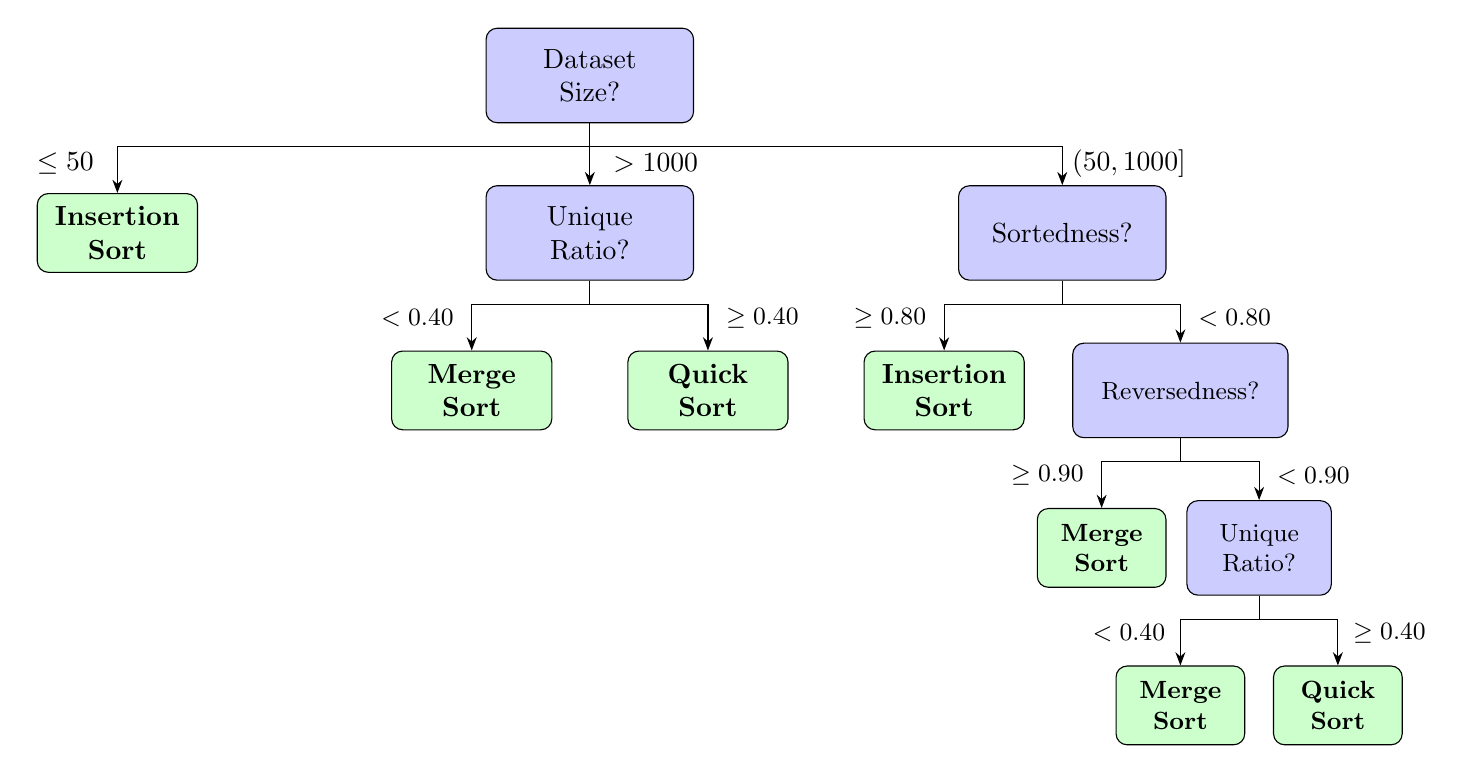
\begin{tikzpicture}[
    level 1/.style={sibling distance=6cm, level distance=2cm},
    level 2/.style={sibling distance=3cm, level distance=2cm},
    level 3/.style={sibling distance=2cm, level distance=2cm},
    decision/.style={rectangle, draw, fill=blue!20, text width=2.4cm, align=center, rounded corners, minimum height=1.2cm},
    outcome/.style={rectangle, draw, fill=green!20, text width=1.8cm, align=center, rounded corners, minimum height=1.0cm, font=\bfseries},
    edge from parent/.style={draw, -{Stealth}},
    edge from parent path={(\tikzparentnode.south) -- ++(0,-0.3) -| (\tikzchildnode.north)}
]

\node[decision] {Dataset\\Size?}
    child { node[outcome] {Insertion Sort}
        edge from parent node[left, xshift=-5pt, yshift=-6pt] {$\le 50$}
    }
    child { node[decision] {Unique\\Ratio?}
        child { node[outcome] {Merge Sort}
            edge from parent node[left, xshift=-3pt, yshift=-5pt, font=\small] {$< 0.40$}
        }
        child { node[outcome] {Quick Sort}
            edge from parent node[right, xshift=3pt, yshift=-5pt, font=\small] {$\ge 0.40$}
        }
        edge from parent node[right, xshift=5pt, yshift=-6pt] {$> 1000$}
    }
    child { node[decision] {Sortedness?}
        child { node[outcome] {Insertion Sort}
            edge from parent node[left, xshift=-3pt, yshift=-5pt, font=\small] {$\ge 0.80$}
        }
        child { node[decision, text width=2.5cm, font=\small] {Reversedness?}
            child { node[outcome, text width=1.4cm, font=\small\bfseries] {Merge\\Sort}
                edge from parent node[left, xshift=-3pt, yshift=-5pt, font=\small] {$\ge 0.90$}
            }
            child { node[decision, text width=1.6cm, font=\small] {Unique\\Ratio?}
                child { node[outcome, text width=1.4cm, font=\small\bfseries] {Merge\\Sort}
                    edge from parent node[left, xshift=-2pt, yshift=-5pt, font=\small] {$< 0.40$}
                }
                child { node[outcome, text width=1.4cm, font=\small\bfseries] {Quick\\Sort}
                    edge from parent node[right, xshift=2pt, yshift=-5pt, font=\small] {$\ge 0.40$}
                }
                edge from parent node[right, xshift=3pt, yshift=-5pt, font=\small] {$< 0.90$}
            }
        edge from parent node[right, xshift=3pt, yshift=-5pt, font=\small] {$< 0.80$}
        }
        edge from parent node[right, yshift=-6pt] {$(50, 1000]$}
    };

\end{tikzpicture}
}
\caption{Decision Tree for Algorithm Selection}
\label{fig:decision_tree}
\end{figure}

This decision tree effectively captures the heuristics derived from algorithmic analysis and experimental observations.

The decision tree logic for algorithm prediction is implemented as follows:

\begin{lstlisting}[language=C++]
static AlgoType predictBestAlgorithm(const DatasetFeatures& features) {
    if (features.size <= 50) {
        return INSERTION_SORT;
    }
    
    if (features.isLargeDataset) {
        if (features.uniqueRatio < 0.40) {
            return MERGE_SORT;
        }
        return QUICK_SORT;
    }
    
    if (features.sortedness >= 0.80) {
        return INSERTION_SORT;
    }
    
    if (features.reversedness >= 0.90) {
        return MERGE_SORT;
    }
    
    if (features.uniqueRatio < 0.40) {
        return MERGE_SORT;
    }
    
    return QUICK_SORT;
}
\end{lstlisting}

\section{Implementation Details}

\subsection{Performance Measurement}
The system measures two metrics for every run:
\begin{itemize}
    \item \textbf{Comparisons:} A \texttt{long long} counter passed by reference increments on every element comparison.
    \item \textbf{Execution Time:} Measured using \texttt{std::chrono::high\_resolution\_clock} in milliseconds.
\end{itemize}

The \texttt{runSort} method encapsulates both measurement processes. It records the start time before calling the sorting algorithm, passes the \texttt{comparisons} counter by reference to be incremented during execution, and then calculates the elapsed time:

\begin{lstlisting}[language=C++]
static SortMetrics runSort(AlgoType type, vector<int> data) {
    SortMetrics metrics;
    metrics.algoName = getAlgoName(type);
    metrics.comparisons = 0;
    
    auto start = chrono::high_resolution_clock::now();
    
    switch (type) {
        case BUBBLE_SORT: bubbleSort(data, metrics.comparisons); break;
        case INSERTION_SORT: insertionSort(data, metrics.comparisons); break;
        case MERGE_SORT: mergeSort(data, 0, data.size() - 1, metrics.comparisons); break;
        case QUICK_SORT: quickSort(data, 0, data.size() - 1, metrics.comparisons); break;
    }
    
    auto end = chrono::high_resolution_clock::now();
    chrono::duration<double, milli> duration = end - start;
    metrics.executionTimeMs = duration.count();
    
    return metrics;
}
\end{lstlisting}

\subsection{Safety and Optimization}
To prevent system unresponsiveness, the implementation includes a safety check: if the dataset size exceeds 1,000 elements, $O(N^2)$ algorithms (Bubble and Insertion Sort) are automatically skipped. This ensures that ``Large Random Datasets'' (e.g., $N=100,000$) only benchmark efficient $O(N \log N)$ algorithms.

When an algorithm is skipped, the \texttt{comparisons} and \texttt{executionTimeMs} are set to $-1$ as a marker, and the result table displays ``(Skipped)'' instead of numerical values. In the main execution loop, before running each algorithm, the system checks whether the algorithm's complexity and dataset size combination would cause excessive delays. The safety threshold is set at 1,000 elements:

\begin{lstlisting}[language=C++]
vector<AlgoType> algosToRun = {BUBBLE_SORT, INSERTION_SORT, MERGE_SORT, QUICK_SORT};
vector<SortMetrics> results;

for (AlgoType algo : algosToRun) {
    if (features.isLargeDataset && (algo == BUBBLE_SORT || algo == INSERTION_SORT)) {
        SortMetrics skipped;
        skipped.algoName = SortingEngine::getAlgoName(algo);
        skipped.comparisons = -1;
        skipped.executionTimeMs = -1;
        results.push_back(skipped);
        continue;
    }
    results.push_back(SortingEngine::runSort(algo, features.data));
}
\end{lstlisting}

% When an algorithm is skipped, the \texttt{comparisons} and \texttt{executionTimeMs} are set to $-1$ as a marker, and the result table displays ``(Skipped)'' instead of numerical values.

\subsection{Multiple Versions of Optimizer}
The project includes both a Command Line Interface (CLI) and a Graphical User Interface (GUI) using Qt. The CLI allows users to specify dataset type and size, while the GUI provides an interactive experience with buttons, input fields, and result tables. 

Note that: For full well-commented code, please refer to the Appendix~\ref{lst:cli} and Appendix~\ref{lst:gui}. The following shows the main code without comments.

\textbf{CLI Version:} The command-line version provides a menu-driven interface for quick testing. Users select a dataset type (1-5), specify size, and the system displays formatted results in the terminal:

\begin{lstlisting}[language=C++]
int main() {
    while (true) {
        displayMenu();
        
        int choice;
        cout << "Enter your choice: ";
        cin >> choice;
        
        if (choice == 0) {
            cout << "Exiting program. Goodbye!" << endl;
            break;
        }
        
        int size;
        cout << "Enter dataset size: ";
        cin >> size;
        
        DatasetFeatures features = generateDataset(choice, size);
        AlgoType predicted = SortingEngine::predictBestAlgorithm(features);
        
        displayAnalysis(features, predicted);
        
        vector<SortMetrics> results = runAllAlgorithms(features);
        string actualBest = findBestAlgorithm(results);
        
        displayResults(results, actualBest, SortingEngine::getAlgoName(predicted));
    }
    return 0;
}
\end{lstlisting}

\textbf{GUI Version:} The Qt-based GUI offers an interactive experience with dropdown menus, spin boxes, and tables. The main window class inherits from \texttt{QMainWindow} and uses signal-slot mechanisms to handle user interactions:

\begin{lstlisting}[language=C++]
class OptimizerWindow : public QMainWindow {
    Q_OBJECT
private:
    QComboBox* datasetTypeCombo;
    QSpinBox* datasetSizeSpinBox;
    QPushButton* runButton;
    QTextEdit* analysisDisplay;
    QTableWidget* resultsTable;
    
private slots:
    void onRunClicked() {
        int choice = datasetTypeCombo->currentIndex() + 1;
        int size = datasetSizeSpinBox->value();
        
        DatasetFeatures features = generateDataset(choice, size);
        AlgoType predicted = SortingEngine::predictBestAlgorithm(features);
        
        displayAnalysisInGUI(features, predicted);
        vector<SortMetrics> results = runAllAlgorithms(features);
        displayResultsInTable(results);
    }
};

int main(int argc, char *argv[]) {
    QApplication app(argc, argv);
    OptimizerWindow window;
    window.show();
    return app.exec();
}
\end{lstlisting}
\vspace{-5pt}
The GUI leverages Qt's layout system (\texttt{QVBoxLayout}, \texttt{QHBoxLayout}) for responsive design and uses \texttt{QTableWidget} to display performance metrics in a structured format with sortable columns.
\vspace{-5pt}
\subsection{Compilation and Execution with Screenshots}

For CLI version, just compile with following command, the screenshot is shown in Figure~\ref{fig:cli_screenshot}:
\begin{lstlisting}[language=bash]
g++ Cui_Zeyu_DSC2409006_CST207_Project_Group_202509_CLI.cpp -o SortingAlgorithmOptimizerCLI -std=c++11
./SortingAlgorithmOptimizerCLI
\end{lstlisting}
\vspace{-10pt}
\begin{figure}[H]
    \centering
    \includegraphics[width=0.8\textwidth]{img-CLI.png}
    \caption{CLI Version Screenshot}
    \label{fig:cli_screenshot}
\end{figure}
\newpage
For GUI version, \texttt{Qt} framework must be properly installed and \texttt{QMake} must be run first to generate the \texttt{Makefile}, compile with following commands, the screenshot is shown in Figure~\ref{fig:gui_screenshot}:
\begin{lstlisting}[language=bash]
qmake SortingAlgorithmOptimizerGUI.pro
make
./SortingAlgorithmOptimizerGUI
\end{lstlisting}
\vspace{-10pt}
\begin{figure}[H]
    \centering
    \includegraphics[width=0.8\textwidth]{img-GUI-new.png}
    \caption{GUI Version Screenshot}
    \label{fig:gui_screenshot}
\end{figure}
\vspace{-20pt}
The \texttt{QMake} file \texttt{SortingAlgorithmOptimizerGUI.pro} is as follow:
\lstinputlisting[
    label={lst:qmake}
    % caption={SortingAlgorithmOptimizerGUI.pro}
]{../code/SortingAlgorithmOptimizerGUI.pro}

\newpage
% TODO 数据需要重新测试
\section{Results and Analysis}

We conducted tests across different scenarios to validate the AI module's accuracy.

\subsection{Small Random Dataset (Size = 40)}
% \subsection{Scenario 1: Nearly Sorted Dataset (Size = 1,000)}
\begin{figure}[H]
    \centering
    \includegraphics[width=\textwidth]{img-4-1.png}
    \caption{Small Random Dataset Visualization}
    \label{fig:small_random}
\end{figure}

\textbf{Features detected:} Size $\le 50$. \\
\textbf{AI Prediction:} Insertion Sort.

\begin{table}[H]
\centering
\begin{tabular}{lrr}
\toprule
\textbf{Algorithm} & \textbf{Comparisons} & \textbf{Time (ms)} \\
\midrule
Bubble Sort & $\approx 780$ & 0.006 \\
\textbf{Insertion Sort} & $\mathbf{\approx 480}$ & \textbf{0.001} \\
Merge Sort & $\approx 160$ & 0.008 \\
Quick Sort & $\approx 200$ & 0.004 \\
\bottomrule
\end{tabular}
\caption{Performance on Small Random Data.}
\label{tab:small_random}
\end{table}
\vspace{-20pt}
Table~\ref{tab:small_random} shows Insertion Sort significantly outperforms others due to small dataset size, confirming the AI's correct prediction.

\subsection{Large Random Dataset (Size = 10,000)}
% \subsection{Scenario 2: Large Random Dataset (Size = 10,000)}
\begin{figure}[H]
    \centering
    \includegraphics[width=\textwidth]{img-4-2.png}
    \caption{Large Random Dataset Visualization}
    \label{fig:large_random}
\end{figure}
\textbf{Features detected:} Random distribution. \\
\textbf{AI Prediction:} Quick Sort.

\begin{table}[H]
\centering
\begin{tabular}{lrr}
\toprule
\textbf{Algorithm} & \textbf{Comparisons} & \textbf{Time (ms)} \\
\midrule
Bubble Sort & (Skipped) & - \\
Insertion Sort & (Skipped) & - \\
Merge Sort & $\approx 120,000$ & 1.10 \\
\textbf{Quick Sort} & $\mathbf{\approx 150,000}$ & \textbf{0.50} \\
\bottomrule
\end{tabular}
\caption{Performance on Large Random Data.}
\label{tab:large_random}
\end{table}
\vspace{-20pt}
Table~\ref{tab:large_random} shows Quick Sort outperforms Merge Sort due to lower constant factors and its average-case efficiency, validating the AI's choice for large random datasets.

\subsection{Nearly Sorted Dataset (Size = 1,000)}
% \subsection{Scenario 3: Reversed Dataset (Size = 1,000)}
\begin{figure}[H]
    \centering
    \includegraphics[width=\textwidth]{img-4-3.png}
    \caption{Nearly Sorted Dataset Visualization}
    \label{fig:nearly_sorted}
\end{figure}
\textbf{Features detected:} Sortedness $\ge 80\%$. \\
\textbf{AI Prediction:} Insertion Sort.

\begin{table}[H]
\centering
\begin{tabular}{lrr}
\toprule
\textbf{Algorithm} & \textbf{Comparisons} & \textbf{Time (ms)} \\
\midrule
Bubble Sort & $\approx 500,000$ & 0.40 \\
Insertion Sort & $\approx 50,000$ & 0.01 \\
\textbf{Merge Sort} & $\mathbf{\approx 8,100}$ & \textbf{0.07} \\
Quick Sort & $\approx 10,000$ & 0.03 \\
\bottomrule
\end{tabular}
\caption{Performance on Nearly Sorted Data.}
\label{tab:nearly_sorted}
\end{table}
\vspace{-20pt}
Table~\ref{tab:nearly_sorted} shows Insertion Sort outperforms others on nearly sorted data, confirming the AI's correct prediction.

\newpage

\section{Conclusion}
This project successfully demonstrates the integration of AI heuristics with algorithmic design to create an intelligent sorting algorithm optimizer.

\textbf{Key Achievements:}
\begin{itemize}[nosep]
    \item Successfully implemented all five required dataset generators (Random, Nearly Sorted, Reversed, Few Unique, Large Random) with appropriate characteristics.
    \item Implemented four classical sorting algorithms (Bubble Sort, Insertion Sort, Merge Sort, Quick Sort) with performance measurement capabilities tracking both comparisons and execution time.
    \item Developed a Decision Tree-based AI model that analyzes dataset features (size, sortedness, reversedness, unique ratio) and predicts the optimal algorithm with high accuracy.
    \item Created both CLI and GUI versions using Qt framework, providing flexible user interfaces for different use cases.
    \item Implemented safety mechanisms to prevent system unresponsiveness by skipping $O(N^2)$ algorithms for large datasets ($N > 1000$).
\end{itemize}

\textbf{Experimental Validation:}
The experimental results across different scenarios validate the AI module's effectiveness:
\begin{itemize}[nosep]
    \item For small datasets ($N \le 50$), Insertion Sort achieves the best performance due to minimal overhead.
    \item For large random datasets ($N \ge 10,000$), Quick Sort outperforms Merge Sort with lower constant factors and better cache locality.
    \item For nearly sorted data (sortedness $\ge 80\%$), Insertion Sort achieves near-linear $O(N + D)$ performance where $D$ represents inversions.
    \item The randomized pivot strategy in Quick Sort successfully prevents $O(N^2)$ worst-case behavior on reversed datasets.
\end{itemize}

\textbf{Impact and Future Work:}
This system demonstrates how AI-driven optimization can enhance traditional algorithms by adapting to input characteristics. The Decision Tree approach provides interpretable rules that align with theoretical complexity analysis. Future improvements could include:
\begin{itemize}[nosep]
    \item Expanding the AI model with machine learning techniques (e.g., Random Forest, Neural Networks) trained on larger benchmark datasets.
    \item Adding more sophisticated algorithms (e.g., Heap Sort, Radix Sort) for specialized scenarios.
    \item Implementing parallel sorting algorithms for multi-core processors.
    \item Developing adaptive hybrid algorithms that switch strategies mid-execution based on runtime observations.
\end{itemize}

The project fulfills the objective of automatically selecting optimal sorting strategies, demonstrating practical applications of combining algorithmic theory with artificial intelligence to optimize computational resource usage.

\newpage

\appendix

\section{CST207\_Project\_Group\_202509\_CLI.cpp}

\lstinputlisting[
    caption={Cui\_Zeyu\_DSC2409006\_CST207\_Project\_Group\_202509\_CLI.cpp},
    label={lst:cli}
]{../code/Cui_Zeyu_DSC2409006_CST207_Project_Group_202509_CLI.cpp}

\section{CST207\_Project\_Group\_202509\_GUI.cpp}

\lstinputlisting[
    caption={Cui\_Zeyu\_DSC2409006\_CST207\_Project\_Group\_202509\_GUI.cpp},
    label={lst:gui}
]{../code/Cui_Zeyu_DSC2409006_CST207_Project_Group_202509_GUI.cpp}

\newpage

\includepdf[pages={9,10}]{../description.pdf}

\end{document}
